\label{37-0508}
\subsection{Proof of Burnside's Lemma}
First, recall Burnside's Lemma: 

\begin{lemma}1
    The number of equivalence classes in $S$ under the action of permutation 
    group $G$ can be calculated to be
    \[ \frac 1{|G|} \sum_{\pi \in G} |\mathrm{fix}(\pi)| \]
\end{lemma}
Recall also the Orbit-Stabilizer Theorem: 
\begin{theorem}2
    For any $s \in S$ with associated permutation group $G$, 
    \[ |\text{Orb}(S)| \cdot |\text{stab}(s)| = |G| \]
\end{theorem}
Now, let us count the orbits/equivalence classes of 2-colored vertices of the
square under the dihedral group $D_4$. Suppose we have red and green as our colors. 
Then the orbits are: 
\begin{itemize}
    \item the all-red coloring 
    \item 3 red, 1 green (in each of the four corners)
    \item 2 red, 2 green, with reds/greens adjacent (4 such colorings)
    \item 2 red, 2 green, with reds/greens at opposite corners (2 such colorings)
    \item 3 green, 1 red (in each of the four corners)
    \item the all-green coloring 
\end{itemize}
There are 6 equivalence classes. This example is helpful for the proof: 
\begin{proof}
    Count the fixed points in the table $S \times G \to S$. Note that 
    the fixed points with $\pi(s) = s$ can be counted in two ways -- counting
    by group elements or by elements of $S$, we see that this is 
    \[ \sum_{\pi \in G} |\mathrm{fix}(\pi)| = \sum_{s \in S} |\text{stab}(s)|, \]
    which, via the Orbit-Stabilizer Theorem we see to be equal to $$\sum_{s \in S} \frac{|G|}{|\text{orb}(s)|}.$$ 
    Partitioning the elements of $S$ into their respective orbits, we can rewrite this
    as 
    \[
        \sum_{O_i \in \text{Orbits}} \sum_{s \in O_i} \frac{|G|}{|\text{orb}(s)|} = 
        |G| \sum_{O_i \in \text{Orbits}} \sum_{s \in O_i} \frac 1{|O_i|} =
        |G| \sum_{O_i \in \text{Orbits}} |O_i| \cdot \frac 1{|O_i|}
    \]
    \[
        = |G| \sum_{O_i \in \text{Orbits}} 1 = |G| \cdot \text{\#orbits}.
    \]
    Dividing both sides by $|G|$, we see 
    \[
        \text{\#orbits} = \frac 1{|G|}\sum_{\pi \in G} |\mathrm{fix}(\pi)|.
    \]

\end{proof}

\subsection{Polya's Enumeration Theorem}
\begin{definition}
    Let $X$ be a set (``vertices'') and $S$ be a set of functions $X \to C$ 
    ($C$ is a set of ``colors''). Let $G$ be a group operating on $X$. We 
    will say two elements $f_i, f_j$ of $S$ are \emph{equivalent} iff 
    there is some $\pi \in G$ such that $f_i(x) = f_j(\pi(x))$ for all $x \in X$. 
\end{definition}
\begin{example}1
    \[ \begin{array}{cc}G & R \\ R & R  \end{array} \cong 
    \begin{array}{cc}R & R \\ G & R  \end{array}\]
    because $H$ acting on the first coloring (viewed as a function) turns it into the second. 

    Explicitly, if we number the vertices as $\begin{array}{cc}1&2 \\3&4 \end{array}$,
    the first coloring is the function $f_1$ with $1 \mapsto G$, $2, 3, 4 \mapsto R$, and
    the second coloring is the function $f_2$ with $3 \mapsto G$, $1,2,4 \mapsto R$. $H$ 
    in cycle notation is the permutation $\pi_H = (13)(24)$. We can check: 
    \[
        f_1(\pi_H(1)) = f_1(3) = R = f_2(1) \quad f_1(\pi_H(2)) = f_1(4) = R = f_2(2)
    \] 
    \[
        f_1(\pi_H(3)) = f_1(1) = G = f_2(3) \quad f_1(\pi_H(4)) = f_1(2) = R = f_2(4)
    \]
\end{example}
\begin{definition}
    The \emph{weight} of the colors is some function $w : C \to \mathcal F$ 
    for some field $\mathcal F$.
\end{definition}
\begin{definition}
    The \emph{weight} $W(f)$ of a function $f : X \to C$ is defined to be $\prod_{x\in X} w(f(x))$. 
\end{definition}
\begin{definition}
    The \emph{inventory} of a set $S$ of functions is $\sum_{f \in S} W(f)$. 
\end{definition}
\begin{example}2
    For the 2-colorings of the square, if we take $w(R) = r$ and $w(G) = g$ 
    (where $r, g$ are some variables that can be added and multiplied), then 
    for the two 2-colorings above, we have that $W(f_1) = r^3 g = W(f_2)$. 

    The inventory of all 2-colorings of a square is 
    \[
        r^4 + 4 r^3g + 6r^2g^2 + 4rg^3 + g^4 = (r+g)^4.
    \]
\end{example}

\begin{definition}
    The \emph{cycle index polynomial} of a permutation group is
    \[
        P_G(x_1, x_2, \dots, x_k, \dots) = 
        \frac 1{|G|} \sum_{\pi \in G} x_1^{b_1} x_2^{b_2} \dots x_k^{b_k} \dots 
    \]
    where $b_k$ is the number of cycles of length $k$ in $\pi$. 
\end{definition}
\begin{example}3
    For the dihedral group $D_4$, where the vertices are labeled $\begin{array}{cc}1&2 \\4&3 \end{array}$:
    $$ e : (1)(2)(3)(4) \to x_1^4 $$
    $$ r_{90} : (2143) \to x_4^1 $$
    $$ r_{180} : (13)(24) \to x_2^2 $$
    $$ r_{270} : (1234) \to x_4^1 $$
    $$ H : (14)(23) \to x_2^2 $$
    $$ V : (12)(34) \to x_2^2 $$
    $$ L : (24)(1)(3) \to x_1^2x_2 $$
    $$ R : (13)(2)(4) \to x_1^2x_2 $$
    So, the cycle index polynomial for $D_4$ is 
    \[ \frac 18 (x_1^4 + 3x_2^2 + 2x_1^2 x_2 + 2x_4). \]
\end{example}
Now, to state Polya's theorem: 
\begin{theorem}
    The inventory of the equivalence classes of functions $f : X \to C$ 
    under the action of permutation group $G$ is given by 
    \[
        P_G(\sum w(x), \sum w^2(x), \sum w^3(c), \dots)
    \]
\end{theorem}
\begin{example}4
    For the square under $D_4$, the inventory is given to be 
    \[ P_G(r + g, r^2 + g^2, r^3 + g^3, r^4 + g^4)\]
    \[ = \frac 18 ((r+g)^4 + 3(r^2 + g^2)^2 + 2(r+g)^2 (r^2 + g^2) + 2(r^4 + g^4))\]
    \[ = g^4 + g^3 r + 2g^2 r^2 + gr^3 + r^4 \]
\end{example}
\begin{corollary}1
    The number of equivalence classes of functions $f : X \to C$ under the 
    action of permutation group $G$ is $P_G(|C|, |C|, |C|, \dots)$
\end{corollary}
\begin{proof}
    Plug in 1 for $w(c)$. So, $w(c) = 1$ for each color. For example,
    in the examples for the square above, take $w(R) = w(G) = 1$.
\end{proof}
\begin{example}5
    The cycle index polynomial of the symmetries of the cube is: 
    \[
        P_G(x_1, x_2, x_3, x_4) = \frac 1{24}(x_1^6 + 3x_1^2 x_2^2 + 6 x_2^3 + 6 x_1^2 x_4 + 8 x_3^2). 
    \]
    Plugging $|C| = n$ into the polynomial, we get the number of equivalence 
    classes of colorings of the cube to be equal to 
    \[ C(n) = \frac 1{24}(n^6 + 3n^4 + 6n^3 + 6 n^3 + n^2) = \frac 1{24}(n^6 + 3n^4 + 12n^3 + 8n^2).  \]
\end{example}

Take this example from chemistry: 
\begin{example}6
    Consider the following tetrahedral structure:
    \begin{center}
        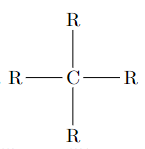
\includegraphics[scale=1]{figures/tetrahedron_chemistry.png}

        $R = \begin{cases} CH_3 & \text{methyl} \\ C_2H_5 & \text{ethyl} \\
            H & \text{hydrogen} \\ Cl & \text{chlorine} \end{cases}$ 
    \end{center}
    Find (a) the number of molecules, and (b) the ones containing $\geq 1$ 
    solitary $H$ atom. It is a chemical fact that these molecules are in 
    fact not planar, but actually tetrahedral. 

    The symmetry group of the tetrahedron has these categories of elements, 
    written in cycle notation: 
    $$ e : (1)(2)(3)(4) : 1$$
    $$ r_v : (1)(234) : 4$$
    $$ r_v^2 : (1)(243) : 4 $$
    $$ r_3 : (12)(34) : 3$$ 
    We can use these to find the cycle index polynomial to be 
    \[ \frac {x_1^4 + 8 x_1 x_3 + 3x_2^2}{12}.\]
    So $C(n) = \frac{n^4 + 11n^2}{12}$. We then see that $C(4) = 36$ and $C(3) = 15$. 
    Using complementary counting we can find the answer to (b) to be $C(4) - C(3) = 21$. 
\end{example}
